\chapter{Design}
\label{design}

\begin{itemize}
\item Develop the overall software architecture

\begin{itemize}
\item Identify major system components

\item Specify interactions between system components

\item Specify system components

\begin{itemize}
\item interfaces

\item semantecs

\end{itemize}

\end{itemize}

\item The Design section should allow a skilled programmer to implement the system

\end{itemize}

NOTES:



\section{theory}
\label{theory}



\section{Training the system}
\label{trainingthesystem}



Since the system bases its decisions on data gathered on the user, the system is essentially trying to mimic user actions at the right times. The system will have three stages :
* The untrained stage where the system is running, but it hasn't yet collected enough data to make intelligent decisions. 

\begin{itemize}
\item The learning stage where there's enough data to attempt to manipulate the switches of the home. We call this the learning stage, because it provides us with a unique opportunity for the system to learn from the user. If the system makes a mistake and the user corrects it, e.g., the system turns off the lights and the user turns it back on, we can use that interaction to train our system further. In this case we can see it as the user punishing the system for making a mistake. The system will then adjust its decision scheme. 

\item After the system has been in the learning stage, it will enter its final stage, which we call the evolution stage. Here the system constantly updates its decision scheme with new data both from monitoring the user, and from being punished for its mistakes. In this stage there is a symbioses between the user and the system where the system reacts to the user and vice versa. $<$Som jeg forstår dette, så adskiller det sig ikke fra learning stage. Tekstmæssigt er forskellen, at her er det også brugeren, der ændrer opførsel. Men det har vel ikke noget med systemets udvikling at gøre. - men sandsynligt.$>$

\end{itemize}

\section{Event patterns}
\label{eventpatterns}

One thing is knowing where the user is, another where the user is headed. By also looking at the preceding interval leading up to an event, it's possible to match that against previously observed patterns, to estimate where the user might be headed.

To determine these pattern we try to make some rules about what to look for. If too long time passes between event, the event are probably not part of the same movement pattern. But what is too long time? $<$god dont let me wait in suspence{\ldots} how long? HOW LONG???!!!$>$

\section{Analyzing the data}
\label{analyzingthedata}

\section{Zones}
\label{zones}

In many cases to cover an entire room with sensors, the sensors end up overlapping in some areas. These overlaps can be used to increase the precision of the sensors. If two sensors triggers shortly after each other, then the user is in the zone where the two sensors overlap. In cases where multiple sensors triggers at the same time, it can be seen as one zone event.

Take (\autoref{zoneimg}) as an example, of three sensors which overlap a bit, and three paths past the sensors a, b and c. The paths b and c should only be observed as zone events by the system. While path a should look something like 1, zone 1 \& 2, 2, zone 2 \& 3, 3. depending on the cooldown of the sensors each event may be multiple times in the pattern.

\begin{figure}[htbp]
\centering
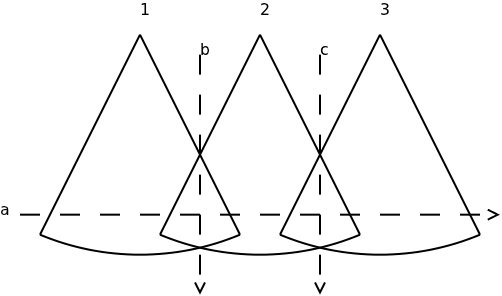
\includegraphics[keepaspectratio,width=\textwidth,height=0.75\textheight]{figures/zone.png}
\caption{Sensors with overlapping zones}
\label{zoneimg}
\end{figure}



\section{Switch and sensor correlation}
\label{switchandsensorcorrelation}

It is beneficial to get a sense of which sensors are near which switches. And we have a lot of statistical data too look at. When a user turns a which on, it most likely because there isn't light where the user intends to be in the immediate future. So it is possible to get an idea of which sensors are near a which, by looking at the interval shortly after a switch is turned on.

$<$TODO maybe talk about that is is less likely that a user will turn on a switch on, and then not enter that room$>$

When flicking a switch off, the user may be leaving the room, or just have entered the room to turn the switch off. Each of the two cases are just as likely as the other, but the sensor events in the interval leaving up to the off event is completely opposite. 

$<$TODO you could possebly look at the interval after it's turned off, and say there are less likely to be in the room, and then try to reduce the correlation for those sensors (NYI)$>$

Based on the statistical data it is possible to generate a table of probability that a sensor is triggered shortly after a switch is turned on, and by extension of that give a idea of wich sensors are in the same room as a switch

\[ P(sensor_i | switch_j , \Delta t) = \frac{\sum 1_{sensor_i} (switch_i, \Delta t) }{\sum switch_j \ events } \]

The indentity function $ 1_{sensor_i} (switch_i, \Delta t) $ is 1 if the sensor is triggered within $\Delta t$ after $switch_j$ is triggered, and is not therefor not counted twice, in the sensor triggeres multiple times after the same switch event.

So to reiterate $ P(sensor_i | switch_j , \Delta t) $ is the probability that $sensor_i)$ fires within $\Delta t$ after $switch_j$ fires.

\begin{table}[htbp]
\begin{minipage}{\linewidth}
\setlength{\tymax}{0.5\linewidth}
\centering
\small
\caption{Correlation table}
\label{ctable}
\begin{tabulary}{\textwidth}{@{}ccccc@{}} \toprule
&sensor 1 $(se_1)$&sensor 2 $(se_1)$&{\ldots}&sensor n $(se_n)$\\
\midrule
switch 1 ($sw_1)$&$P(se_1 | sw_1, \Delta t)$&$P(se_2 | sw_1, \Delta t)$&{\ldots}&$P(se_n | sw_1, \Delta t)$\\
switch 2 ($sw_2)$&$P(se_1 | sw_2, \Delta t)$&$P(se_2 | sw_2, \Delta t)$&{\ldots}&$P(se_n | sw_2, \Delta t)$\\
$\vdots$&$\vdots$&$\vdots$&$\ddots$&$\vdots$\\
switch m ($sw_m)$&$P(se_1 | sw_m, \Delta t)$&$P(se_2 | sw_m, \Delta t)$&{\ldots}&$P(se_n | sw_m, \Delta t)$\\

\bottomrule

\end{tabulary}
\end{minipage}
\end{table}

